\chapter{The Standard Model}
\label{chap:I-1-standard-model}

  The standard model provides a classification and description of the subatomic particles that compose our universe and their interactions. It describes both the particles of matter called fermions, which are subdivied among quarks and leptons, and the force carriers named bosons. Figure \ref{fig:I-1-sm-particles} gives a schematic view of the particle content of the standard model and the ways they are classified. Quarks and leptons are further divided into three generations, with identical properties but increasing mass, from which the first constitutes the everyday matter while the two others quickly decay towards lower generations. The interaction of fermions with each other is carried out through the exchange of bosons. Gluons are the carriers of the strong force and interract solely with themselves and quarks as described by QCD. The photon, responsable for electromagnetism couples to all charged particles while the $ W^\pm $ and $ Z $ bosons couple to all particles except gluons as described by EWK. Finally, the Higgs boson as previously stated is the manifestation of the Higgs mechanism at the origin of mass. \\

	\begin{figure}[h!]
		\centering
		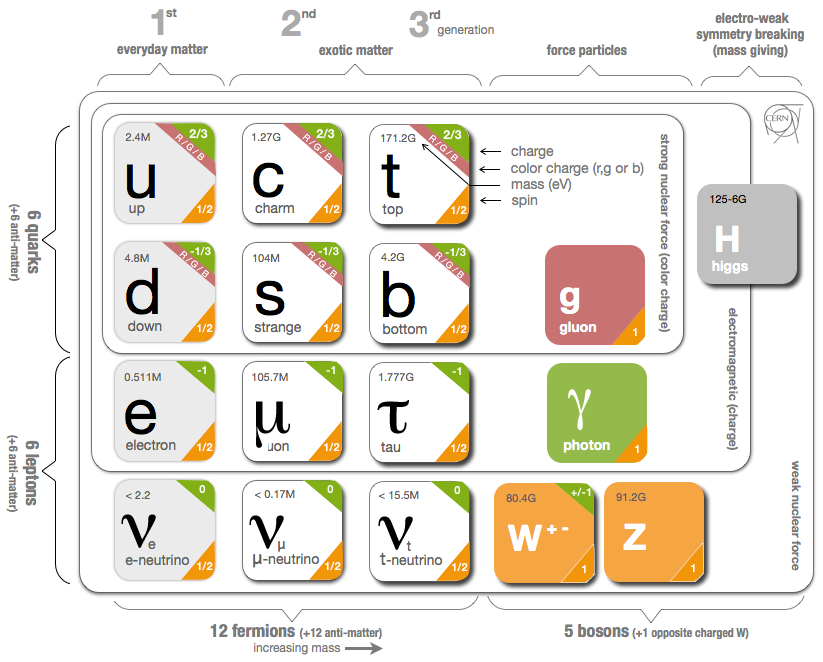
\includegraphics[width = 0.8 \textwidth]{img/I-1/sm-particles.png}
		\caption{Overview of the elementary particles as described by the standard model. Everyday matter is composed of the first generation of quarks and leptons to which two generations of heavier declinaisions are added. Gauge bosons or force particles are the carriers of the interactions between the other particles. The Higgs boson is the manifestation of the mechanism that gives mass to particles [CERN].}
		\label{fig:I-1-sm-particles}
	\end{figure}

  Besides classifying particles, the standard model also provide as strong mathematical model built on top of quantum field theory and gauge invariance. The gauge group of the theory is $ SU(3)_C \otimes SU(2)_L \otimes U(1)_Y $, where $ SU(3)_C $ and $ SU(2)_L \otimes U(1)_Y $ are respectivly the symetry groups of the QCD and EWK sectors. Quarks and leptons are represented as fermionic fields within the Lagrangian of the model while bosons arise from the invariance of the Lagrangian under local gauge transformations.

  \section{Electroweak Theory}

    A local transformation of a fermionic field $ \psi $ under the gauge group of the EWK sector of the standard model $ SU(2)_L \otimes U(1)_Y $ can be written as
    \begin{equation}
      \psi \rightarrow \psi' = \exp\left( \frac{i}{2} g_W \Lambda^k(x) T^k \right) \exp\left( \frac{i}{2} g_W' \alpha(x) Y \right) \psi ,
    \end{equation}
    where $ g_W $, $ \Lambda^k(x) $, and $ T^k $ are respectivly the gauge coupling, local rotation parameters, and represenation of the $ SU(2)_L $ weak isospin algebra and $ g_W' $, $ \alpha(x) $, and $ Y $ are their $ U(1)_Y $ hypercharge algebra counterparts. To preserve the invariance of the Lagrangian of a free massless field $ \psi $,
    \begin{equation}
      \mathcal{L} = i \bar{\psi} \gamma^\mu \partial_\mu \psi ,
    \end{equation}
    the partial derivate $ \partial_\mu $ must be rewriten as a covariant derivate
    \begin{equation}
      D_\mu = \partial_\mu + i g_W W^k_\mu T^k + i g_W' B_\mu Y ,
    \end{equation}
    where $ W^k_\mu $ and $ B_\mu$ are the emerging gauge fields associated to $ SU(2)_L $ and $ U(1)_Y $. The gauge invaratiant Lagrangian thus becomes
    \begin{equation}
      \mathcal{L} = i \bar{\psi} \gamma^\mu D_\mu \psi - \frac{1}{4} W^i_{\mu \nu} W^{i \mu \nu} - \frac{1}{4} B_{\mu \nu} B^{\mu \nu} ,
    \end{equation}
    where $ W^i_{\mu \nu} $ and $ B_{\mu \nu} $ are the field strength tensors of the $ W^i_\mu $ and $ B_\mu $ gauge fields given by
    \begin{align}
      W^i_{\mu \nu} & = \partial_\mu W^i_\nu - \partial_\nu W^i_\mu - g_W \epsilon^{ijk} W^j_\nu W^k_\mu \ \text{and} \\
      B_{\mu \nu} & = \partial_\mu B_\nu - \partial_\nu B_\mu ,
    \end{align}
    where $ \epsilon^{ijk} $ is the totaly antisymetrical tensor. Interaction terms between the fermionic field $ \psi $ and $ W^i_\mu $ and $ B_\mu $ as well as self-interacting gauge fields terms have emerged from the necessity of the invariance of the theory under local transformations. \\

    The physical fields of the photon $ A_\mu $ and the weak interaction bosons $ W^\pm_\mu $ and $ Z_\mu $ are linear combination of the $ B_\mu $ and $ W^i_\mu $ gauge fields. This is a consequence of the higgs mechanism that will be described in Section \ref{sec:I-1-higgs-mechanism}

    Each fermion can couple differently to the gauge fields according to the representation of the $ SU(2)_L $ group they are part of. To determine the coupling constants it is important to separate each fermionic field into its left-handed and right-handed components such that
    \begin{equation}
      \psi = \psi_L + \psi_R \equiv \gamma_L \psi + \gamma_R \psi ,
    \end{equation}
    with
    \begin{align}
      \gamma_{L/R} & = \frac{1}{2} \left( 1 \mp \gamma_5 \right) \ \text{and} \\
      \gamma_5 & = \frac{1}{24} \epsilon^{\mu \nu \rho \sigma} \gamma_\mu \gamma_\nu \gamma_\rho \gamma_\sigma ,
    \end{align}
    where $ \gamma_\mu $ are the Dirac matrices. It has been showed experimentatly that only left-handed particles interact with the $ SU(2)_L $ group, meaning that right-handed particles are part of the singlet representation of the group. Left-handed particles are part of the doublet representation in which they are grouped.


  \section{Quantum Chromodynamics}

  \section{The Brout-Englert-Higgs Mechanism}
  \label{sec:I-1-higgs-mechanism}

  \section{Beyond the Standard Model}
